\section{Theory}
\label{section:theory}
This section covers the theory behind different aspects of the city generation tool of this thesis, namely: PCG approaches and methods for generating certain city elements as well as the surrounding terrain and a few words about developing extensions for Unity.

\subsection{Constructive and Generate-And-Test approaches to PCG}
The difference between constructive algorithms for PCG and generate-and-test algorithms is that the former only involves the actual generation of the content; once the content has been generated, the process is done. The latter, however, also involves testing the content and making sure that it meets all specified requirements. If it does not, it is ignored and the process starts over and repeats until all criteria are met \cite{search-based_pcg}.

\subsection{The Search-based approach to PCG}
The search-based approach to PCG is based on the previously mentioned approach called "generate-and-test". The difference is that generated content in the search-based approach is graded for its quality, unlike generate-and-test, where it is instantly discarded if not optimal. The grading is done with fitness functions (also called evaluation functions) that determine how suitable the content is in the context. The generation of content depends on previous results and fitness scores to increase the content quality \cite{search-based_pcg}. The search-based approach consists of three main parts: the search algorithm, the content representations and the evaluation functions \cite[pp. 17-20]{shaker2016procedural}.

\subsubsection{Content representations}
Content representations can be interpreted as blueprints, defining how different types of content are to be generated \cite[p. 18]{shaker2016procedural}. A game level, for instance, probably has to contain certain elements to fit into the game that is being developed. The content representation can therefore contain data about what is required and can then be used to generate actual levels. 

Togelius and Shaker describe content representations in the terms of "genotypes" and "phenotypes" in the context of evolutionary search algorithms. The former is what is used to generate content and the latter is the actual generated content, derived from the genotype \cite[pp. 18, 20]{shaker2016procedural}. Referencing the earlier example about game levels; the genotype would be the data about what is required in the level and the phenotype would be the generated level itself.

\subsubsection{Evaluation functions}
Evaluation functions determine how well-generated content fits into the context. An example of this is a game level that has been generated and then evaluated to verify that it is possible to beat and that it is neither too easy nor hard to play. There are at least three types of evaluation functions: direct, simulation-based and interactive \cite[pp. 18-24]{shaker2016procedural}.

% Direct
Evaluation functions that directly calculate fitness values based on the generated content's attributes are called "direct". Such functions can either be driven by theory or by data. The former means that the evaluation is based on theories about how players will experience the content. The latter means that the evaluation is based on collected data and statistics about player experience \cite[p. 23]{shaker2016procedural}.

% Simulation-based
As the name suggests, simulation-based evaluation functions involve simulating the use of generated content to evaluate their respective fitness values. The simulation is done by utilizing AI agents that for example play a generated game level to make estimations. Agents can either be dynamic or static, meaning that they either adapt during the simulation or not \cite[pp. 23-24]{shaker2016procedural}.

% Interactive
Evaluation functions can also be based on human interaction, meaning that human actions can determine the fitness of generated content. An example is giving different fitness values to generated weapons in games, depending on how much they are used by actual human players \cite[p. 24]{shaker2016procedural}.

\subsubsection{Search Algorithms}
There are different types of search algorithms, such as: Evolutionary, exhaustive, random and solver-based. Togelius and Shaker describes an evolutionary search algorithm where the number of generation surviving ''individuals'' (content) is represented by $\mu$ and where the number of ''offspring'', derived from the previous generation, is represented by $\lambda$. The sum of these variables is the total size of the content population when generating. The algorithm consists of eight steps, where only the second one is optional \cite[p. 18-20]{shaker2016procedural}:

\begin{enumerate}
    % Step 1: Initialization
    \item A population with the size of $\mu + \lambda$ has to be initialized in order to generate anything. Since this is the initialization step and is only executed once at the very start of the algorithm, this can be done in any way that is deemed appropriate in the context. The initial population can for example consist of individuals that are man-made, from earlier uses of the algorithm or generated at random.
    % Step 2: Shuffle the population (start of a generation)
    \item Optionally shuffle the population in order to avoid loss-of-gradient situations \cite{shaker2016procedural}, meaning that some subpopulations otherwise could start dominating others \cite{Spatial-Embedding-and-Loss-of-Gradient}.
    % Step 3: Evaluate individuals
    \item The fitness for each individual content is calculated to a numeric value by using it as a parameter in an evaluation function.
    % Step 4: Sort by fitness
    \item The whole population is sorted by the fitness in an ascending order.
    % Step 5: Discard bad individuals
    \item Since $\mu$ is the number of surviving individuals after a generation, a total of $\lambda$ individuals has to be discarded. The ones getting ''killed'' have the worst fitness scores of the population and are therefore not fit to generate any offspring for the next generation.
    % Step 6: Replace the discarded individuals with copies of good ones
    \item The discarded individuals are replaced by copies of the ones with higher fitness scores. Depending on the proportions between $\mu$ and $\lambda$, some elite individuals might not get copied at all or might be copied several times in order to reach the number of $\lambda$ copies, i.e., the population size does not change.
    % Step 7: Mutate some individuals
    \item A number of $\lambda$ individuals are randomly chosen to be mutated (modified) in arbitrary ways. An example of a mutation type is Gaussian mutation.
    % Step 8: Choose to stop or to continue
    \item Depending on if an individual is deemed good enough, based on its fitness score, the algorithm is stopped. It is also stopped if the number of executed iterations is equal to a specified maximum. The algorithm otherwise repeats everything from the second step and thus starts a new generation of individuals.
\end{enumerate}

\subsection{Terrain generation}
A common feature in games is varying terrain which is used to create interesting worlds to explore or sometimes being an integral part of the gameplay.

\subsubsection {Noise functions}
For generating terrain features such as heights, the most common approach is to generate an intensity map represented by a 2D matrix containing the brightness of each pixel \cite[pp. 58-59]{shaker2016procedural}. This can then be used to determine the different heights of the terrain through displacement mapping. An initial attempt at creating such a map could be to assign random values in the matrix as displayed in figure \ref{fig:random-noise} but in the case of terrain this would look like random spikes which would not be suitable for a game environment. To combat this, a type of gradient noise can be used, which was formally described by Ken Perlin in 1985~\cite{image-synthesizer} to generate more realistic looking textures compared to what was available at the time. This method was later improved by Perlin in 2001 where he introduced "simplex noise"~\cite{improving-noise} as seen in figure~\ref{fig:simplex-noise}. Compared to classic Perlin noise this improved algorithm scales to higher dimensions with less computational overhead and is easier to implement in hardware. 

To generate simplex noise in two dimensions, space is divided into simplexes (triangles in this case), where pseudo-random gradients are placed at the corner of each simplex. For every point in the space, the contribution of each simplex is calculated based on the \say{multiplication of the extrapolation of the gradient ramp and a radially symmetric attenuation function.}~\cite{simplex-demystified}.

The issue of using noise functions is that every location is independent of the others, which might make it feel like there is not enough uniqueness for a game environment. Multiple noise maps, controlling different aspects of the terrain, can, however, be used together to create, for example, overhangs and caves, thus making the terrain more interesting.

\begin{figure}[H]
\centering
\begin{subfigure}{.3\linewidth}
  \centering
  
\includegraphics[width=1\linewidth]{random-noise.png}
  \caption{Random noise}
  \label{fig:random-noise}
\end{subfigure}
~
\begin{subfigure}{.3\linewidth}
  \centering
  
\includegraphics[width=1\linewidth]{simplex-noise.png}
  \caption{Simplex noise}
  \label{fig:simplex-noise}
\end{subfigure}
\caption{Two types of noise}
\end{figure}

\subsubsection{Using Agents}
While the inherent randomness of PCG methods like Perlin noise is what makes them desirable, it can often be to the detriment of customizability. Designers can tailor their terrain to some degree, but only on a global level through the adjustment of a set of parameters. Agent-based terrain generation is an alternative which retains customizability while also providing features expected of PCG, such as randomness, unpredictability, speed, and so on \cite[64]{shaker2016procedural}.

Professors Jonathon Doran and Ian Parberry from The University of North Texas describe a way of procedurally generating terrain through software agents \cite{agentbasedTerrain}. Their method is based on five different types of agents. These agents work concurrently to simulate natural phenomena by sensing their environment and changing it at will. Designers can influence the generation of terrain by adjusting the number of agents of each type, or by changing their lifespan by restricting the number of actions they can perform. Once the maximum number of actions is reached, the agent becomes inactive.

Agents can modify the environment by performing three main tasks:

\begin{itemize}
    \item Coastline: The first phase in which multiple agents generate the main shape of the terrain.
    \item Landform: In the next phase more agents are employed to generate the more detailed features of the land. These include lowlands, beaches, and the details of mountains. The agents work simultaneously.
    \item Erosion: In the last phase, pieces of the terrain are chipped away to create rivers. The number of rivers depends on the number of agents.
\end{itemize}
Each phase contains several different types of agents; these include, but are not limited to: coastline agents, smoothing agents and beach agents. The coastline agents generate the rough parts of the environment, while the smoothing agents eliminate any resulting rapid elevation changes. After smoothing, beach agents traverse the shoreline, creating sandy areas near bodies of water.

\begin{figure}[H]
    \centering
    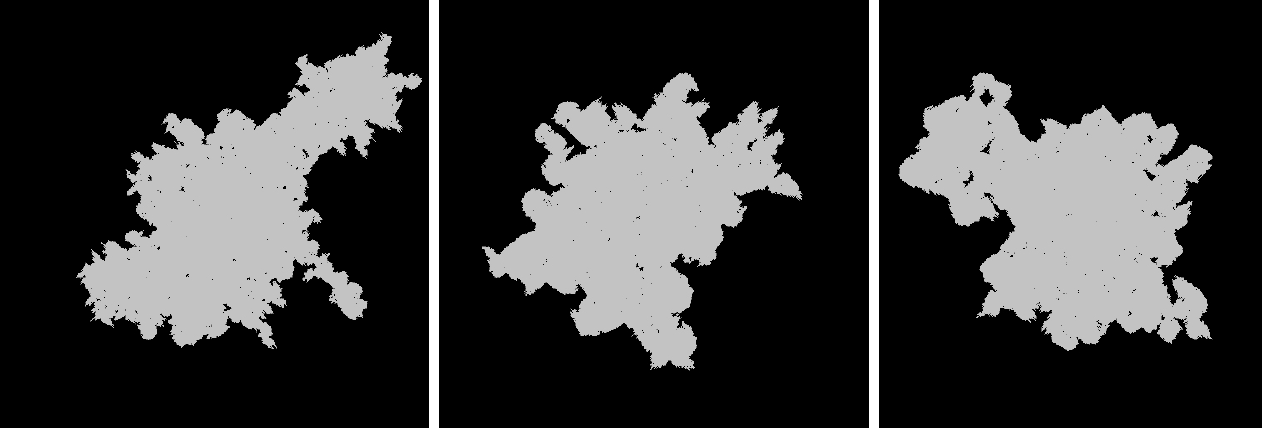
\includegraphics[width = 1\linewidth]{Planning report/images/coastline.PNG}
    \caption{Coastline generated by coastline agents with small, medium and large action sizes.}
    \label{fig:coastline}
\end{figure}
\begin{figure}[H]
    \centering
    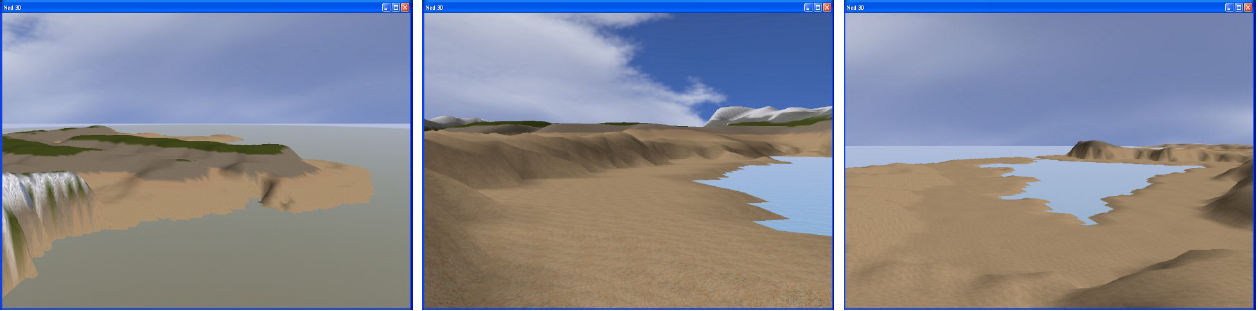
\includegraphics[width = 1\linewidth]{Planning report/images/beach.PNG}
    \caption{Beaches produced by beach agents with small, medium and large beach widths.}
    \label{fig:beach}
\end{figure}

By defining the agents and their sets of parameters, the generation of terrain can be suited to one's needs, and also remain unpredictable through the use of random seed numbers.

\subsection{Road generation}
This section will discuss different algorithms as related to the generation of road networks in a city environment.

\subsubsection{L-systems}
An early candidate for generating road networks was Lindenmayer Systems. L-systems are a special case of generative grammars and are typically used to generate visualizations of vegetation. Though they were introduced to model natural structures, they have also been used in city generation algorithms \cite{yoav-pascal}. 

% Grammars
Grammars are a set of symbols with rewrite rules that replace each symbol in the string with whatever symbols that rule dictates. The string of a grammar consists of terminals, non-terminals and an axiom, which is the initial string. A grammar may also associate parameters with rewriting rules, to modify certain properties of the result \cite{graphical_l-systems}. Rules in a non-deterministic grammar may either decide randomly which valid replacement should occur or use the parameters to determine which rule is the best fit, while deterministic ones only have a single derivation \cite[p. 75]{shaker2016procedural}. 

% L-systems
A defining feature of L-systems is that they rewrite the symbols in a given string in parallel each iteration. L-systems are not limited to the strict representation of strings; graphs and other objects may be represented by an L-system as well \cite[p. 75-79]{shaker2016procedural}. A grammar such as an L-system will generally consist of two parts when used for procedural modelling: the rewriting algorithm and an interpretation \cite{graphical_l-systems}. The interpreter is what will build a graphical representation of the generated data (such as vertices), and thus produce the model itself.

A simple, deterministic L-system: \\*
\begin{align*}
    &Rules: \\
    &\qquad A \to AF \\
    &\qquad F \to Ff \\\
    &Axiom: AF \\\
    &Iteration 1: 	AAFFf \\
    &Iteration 2: 	AAAFFFFff \\
    &Iteration 3: 	AAAAFFFFFFfff
\end{align*}

% Extensions
While L-systems are mostly used for generating graphical representations of plants \cite{SpeedTree}, various extensions to the base grammar have been developed for different purposes within procedural generation algorithms. For example, in previous work by Müller and Parish \cite{yoav-pascal}, a different version of L-systems was used to generate road networks of different types for city generation. The extended system with the same authors used constraints and goals to model the road network, allowing some customization and modularity to be introduced. In that algorithm, the goals set the parameters according to what input data is given, in this case maps over statistics such as population density or city grid data. This allows the generator to produce specific street patterns \cite{yoav-pascal}.

Another possible method to explore is Voronoi diagrams, which has many application areas and could be used for determining the position of the roads.



% ---------------------
\subsection{Urban cities and street patterns}
% city in PCG
Real cities are built up through many generations and have deep cultural roots when it comes to architecture to form the surroundings, such as parks, roads, public transportation, policies, hospitals and styles of its buildings \cite{CityArchitecture}. One can study urbanization of a larger city for insight on city developments when populations are increased, this is called Large-scale Urban Development (LUD) \cite{UrbanCity}. LUDs are a way of making sure that a growing population has housing and its housing is developed with the environment in mind. Buildings of today are generally taller than before, meaning that they can house more people than older buildings on the same area \cite{UrbanCity}.

The street pattern can have an impact on the type of city that is formed, depending on if the newer take on streets, cul-de-sac, or the older grid system gridiron is used. Cul-de-sac is explained like this in an article by Paul K. Asabere: \say{The cul-de-sac (or culs-de-sac in French) is essentially a dead-end street with a turn- around at the end for cars.} \cite{streets_pattern}. The article goes on, explaining the flexibility of cul-de-sac and creative ways to arrange homes. The cul-de-sac can also reduce the amount of pedestrians and bicycles, which is why it is popularly used in newly produced neighborhoods, where the roads do not have to be connected. \say{The gridiron (or grid) came to America from various European sources, taking different forms in New Haven, Philadelphia, Savannah, New Orleans, and Canadian cities such as Halifax.} \cite{streets_pattern}. The use of the grid has more simplicity to it as it is more economical. The name gridiron comes from the layout which is made up by rectangular lots.

\begin{figure}[H]
\centering
\begin{subfigure}{.4\linewidth}
  \centering
  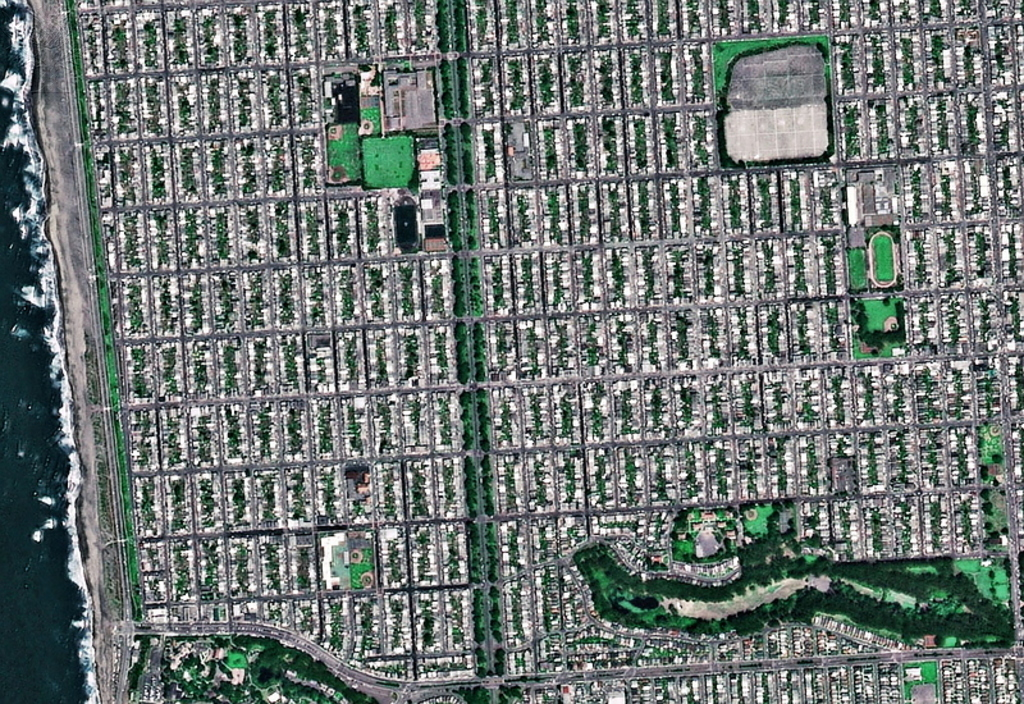
\includegraphics[width=1\linewidth]{Planning report/images/grid_pattern.jpg}
  \caption{Gridiron}
  \label{fig:street_pattern}
\end{subfigure}
~
\begin{subfigure}{.4\linewidth}
  \centering
  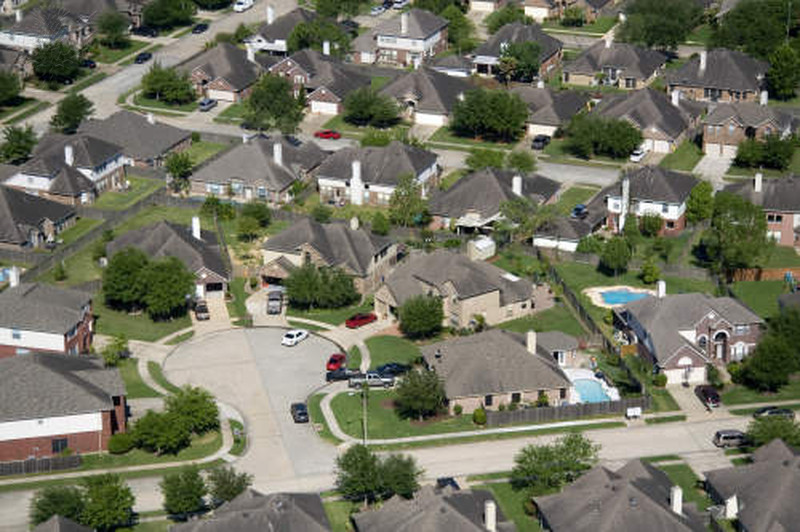
\includegraphics[width=1\linewidth]{Planning report/images/culdesac.jpg}
  \caption{Cul-de-sac}
\end{subfigure}
\caption{Street patterns}
\label{fig:both_pattern}
\end{figure}

\newpage
\subsection{Unity Editor Scripting}
Creating extensions to the Unity editor can be done with editor scripting. Some examples of what can be added to the workflow are custom windows, menu controls of different kinds. New functionality can also be added to the scene view \cite{unity-extending-editor}. There is an official Unity API for editor scripting which is well documented by Unity Technologies \cite{unity-editor-docs}.